\documentclass[a4paper,12pt]{ltjsarticle}

% パッケージ
\usepackage{graphicx}
\usepackage{amsmath, amssymb}
\usepackage{xcolor}
\usepackage{geometry}
\usepackage{enumitem}
\usepackage{hyperref}
\usepackage{luatexja-fontspec}

% フォント設定
\setmainjfont{IPAexMincho}
\setmainfont{Times New Roman}
\setsansjfont{IPAexMincho}
\setsansfont{Times New Roman}

% レイアウト
\geometry{margin=25mm}
\setlist[itemize]{label=--, leftmargin=2em}
\setlist[enumerate]{leftmargin=2em}

%====================
% 強調用コマンド
%====================
\newcommand{\important}[1]{\textcolor{blue}{\textbf{#1}}}

\begin{document}

%====================
% タイトルブロック
%====================
\begin{center}
  {\huge 進捗報告（ver.37）}\\[1em]
  {\large \today}\\
  {\large 千葉工業大学大学院 学習工学研究室}\\
  {\large 内山 裕太}
\end{center}

\vspace{2em}

%====================
\section{進捗概要}
\begin{itemize}
  \item 数学学習の分野調べ
  \item 自身の研究テーマの確定
  \item それっぽいシステムの開発（これから変えていく）
\end{itemize}
\newpage

%====================
\section{進捗詳細}
\subsection*{数学学習の分野調べ}
数学学習を題材とした研究がどのくらい，どのようにされているのかを調査した．結果としては，\href{https://www.jstage.jst.go.jp/browse/jasme/29/0/_contents/-char/ja}{\important{全国数学教育学会}}に面白そうな研究がたくさんあることが分かった．\\

この学会では「研究」をメインに扱っているらしく，別の組織で\important{数学教育学会}もあるらしい．こちらは実践も重要視しているらしく，実際の数学教員なども多く在籍しているらしい．\\

今回は全国数学教育学会の学会誌（数学教育学研究），日本数学教育学会誌の中から以下のものをリストアップした

\begin{enumerate}
  \item \href{https://www.jstage.jst.go.jp/article/jjsme/65/3/65_13/_pdf/-char/ja}{中西知真紀, 国宗進, 家田晴行, 榎戸章仁, 春日龍郎, 金児正史, 小関熙純, 東風谷幸広, 山下国広: 図形における論証指導について, 日本数学教育学会誌, Vol. 65, No. 3, pp. 13-24, 1983}
  \item \href{https://www.jstage.jst.go.jp/article/jasme/27/1/27_33/_pdf/-char/ja}{渡邊慶子, 岡崎正和: 証明言語の生成とふり返りによる定理と証明の相互理解 ―場合分けのある証明に着目して―, Vol. 27, No. 1, pp.33-46, 2021}
  \item \href{https://www.jstage.jst.go.jp/article/jjsme/104/1/104_2/_pdf/-char/ja}{近藤裕: 算数・数学科における「説明・証明」の能力に関する研究, Vol. 104, No. 1, pp. 2-12, 2022}
  \item \href{https://www.jstage.jst.go.jp/article/jasme/3/0/3_KJ00008199223/_pdf/-char/ja}{長谷川順一, 三井誠弦: 中学生の証明問題解決過程の分析, Vol. 3, pp. 137-146, 1997}
  \item \href{https://www.jstage.jst.go.jp/article/jjet/42/Suppl./42_S42092/_pdf/-char/ja}{濱田さとみ, 鷹岡亮, 横山誠: 中学校数学科合同証明を対象とした証明構造理解支援Webアプリの開発と有用性検討, 日本教育工学会論文誌, Vol. 42, No. Suppl, pp. 169-172, 2018}
  \item \href{https://www.jstage.jst.go.jp/article/jjsme/69/11/69_23/_pdf/-char/en}{磯田正美: 体系化の立場から見た中2の図形指導, 日本数学教育学会誌, Vol. 69, No. 11, pp. 23-32}
  \item \href{https://www.jstage.jst.go.jp/article/jasme/23/2/23_141/_pdf/-char/ja}{宍戸建太, 岡崎正和: 図形の証明の構成過程におけるジェスチャーの役割に関する研究, 全国数学教育学会誌 数学教育学研究, Vol. 23, No. 2, pp. 141-149, 2017}
  \item \href{https://www.jstage.jst.go.jp/article/jjsme/77/11/77_17/_pdf/-char/ja}{垣花京子, 清水克彦: 図形の証明問題での測定値の役割 -コンピュータ環境下における生徒の活動分析を通して-, 日本数学教育学会誌, Vol. 77, No. 11, pp. 17-22}
\end{enumerate}

現在は上記の文献を読みつつ，自身のやりたい内容の必要性や新規性について考えている段階

\subsection*{自身の研究テーマの確定}

\subsection*{それっぽいシステムの開発}
自分の想像するシステムを簡単に構成してみた\\
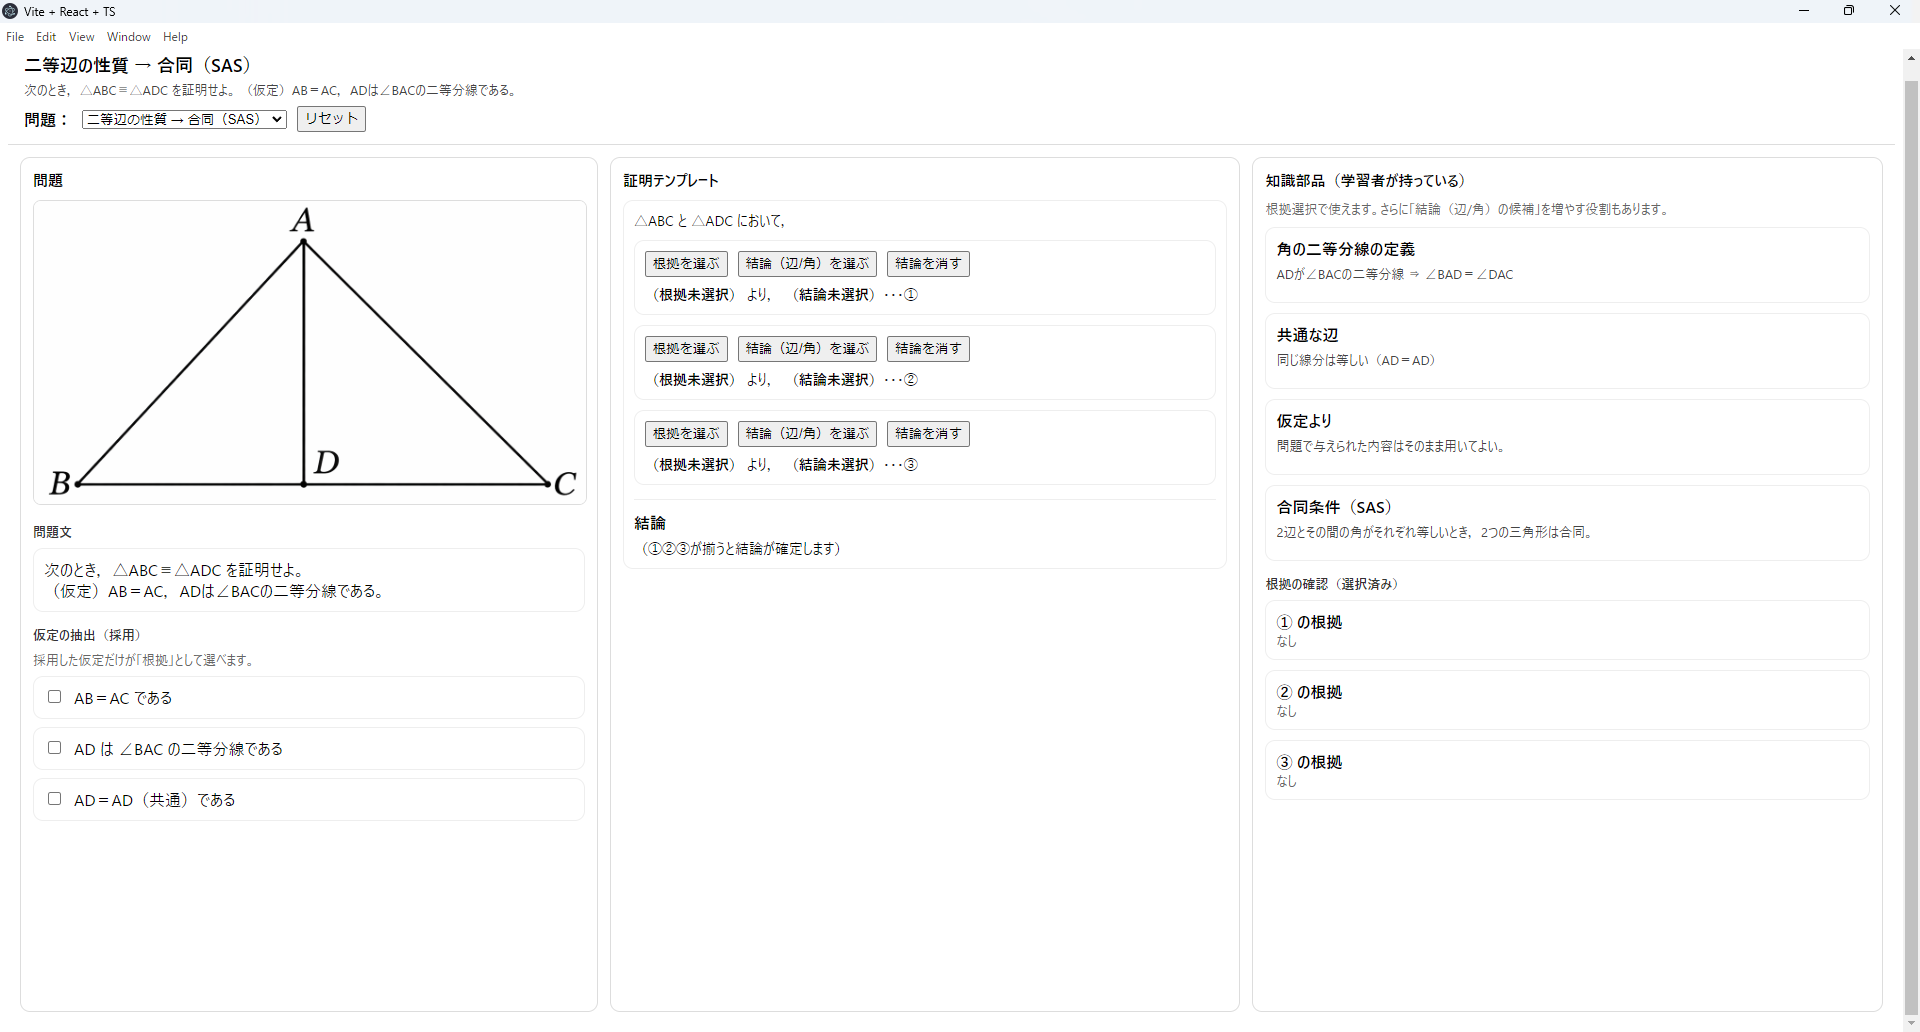
\includegraphics[width=\linewidth]{figs/20260306/system1.png}

%====================
\section{問題点・課題}
\begin{itemize}
  \item 
\end{itemize}

%====================
\section{今後の予定}
\begin{enumerate}
  \item 
\end{enumerate}

%====================
\section*{雑談}
\begin{itemize}
  \item 
\end{itemize}

%====================
\section*{備考・メモ}
\begin{itemize}
  \item 
\end{itemize}

\end{document}
